
\documentclass[a4paper,12pt]{article} 

\usepackage[utf8]{inputenc}
\usepackage[spanish]{babel}
\usepackage{amsmath}
\usepackage{amsfonts}
\usepackage{amssymb} 

\usepackage{graphicx} 			%graficos
\usepackage[colorlinks=true, linkcolor=black, citecolor=black, urlcolor=blue]{hyperref} 	
\usepackage{wrapfig}
\usepackage{enumitem}
\usepackage{fancyhdr}
\usepackage{float}
\usepackage{eurosym}
\usepackage{color}
\usepackage{titling}
\usepackage{lipsum}
\usepackage{tocbibind}
\usepackage{longtable,multirow,booktabs}
\usepackage{multicol}

\usepackage[left=3cm,right=3cm,top=3cm,bottom=4cm]{geometry}		%margenes para documento


\pagestyle{fancy}													% estilo del estlo de pie cabezera


%%% Para las cabeceras
\newcommand{\hsp}{\hspace{20pt}}
\newcommand{\HRule}{\rule{\linewidth}{0.5mm}}
\headheight=50pt


\newcommand{\vacio}{\textcolor{white}{holacaracola}} 			%comando para dar un texto 

% Color azul para algunos 
% textos de la portada
\definecolor{azulportada}{rgb}{0.16, 0.32, 0.75}				%color azul para una ciertas letras


%%%% Azul para textos de headings
\definecolor{azulinterior}{rgb}{0.0, 0.2, 0.6}

%====================================Datos del proyecto
\title{Sistemas de Control de Versiones}				%titulo del proyecto
%%%% AUTOR
\author{Mamani Yucra Alexander\\ \vspace{0.3cm}Mamani Yucra Alexander\\ \vspace{0.3cm}Mamani Yucra Alexander}
%%%%%%%%%%%%%%%%
%%%%%% DIRECTOR DEL TRABAJO
%%%%%%% Cambiar el nombre siguiente
\newcommand{\director}{Ing Andy Cepedes }				%director



\begin{document}

\begin{titlepage} %%%%% Aquí no hay que tocar nada.
	%%%% Las siguientes instrucciones generarán automáticamente
	%%%% la portada de tu proyecto.
	%%% Cambio de la estructura de esta página
\newgeometry{left=0.6cm,top=1cm,bottom=1.2cm}

\fbox{\parbox[c]{18.5cm}{  												%margen de la caratula 
\begin{center}
\vspace{1.5cm}
{\fontfamily{phv}\fontsize{20}{5}\selectfont{\textbf{UNIVERSIDAD TÉCNICA DE ORURO}}}\\	
[2em]

{\fontfamily{phv}\fontsize{16}{4}\selectfont{\textbf{FACULTAD NACIONAL DE INGENIERÍA}}}\\	
[4em]


% Autor del trabajo de investigación
%\textcolor{azulportada}{\fontfamily{phv}\fontsize{16}{5}\selectfont{\theauthor}}\\ [1cm]
% Título del trabajo

%{\Huge\textbf{\thetitle}}\\												%titulo opcional [1cm]																		% un centmetro de vertical


\includegraphics[width=5.5cm]{logosanmateo.png}								%importamos una imagen
\\[1cm]

{\fontfamily{phv}\fontsize{16}{4}\selectfont{TRABAJO DE INVESTIGACIÓN}}\\			%tiyulo de la portada
%\textcolor{azulportada}
[1cm]
{\fontfamily{phv}\fontsize{20}{5}\selectfont{\textsc{\thetitle}}}\\
[2cm]
Presentado por :
\vspace{0.5cm}

\begin{minipage}[b]{6cm}
	\begin{center}
		Univ. Alexander Mamani\\
		FNI\\
		Oruro\\
		akeymy4@gmail.com
	\end{center}
\end{minipage} \hfill \begin{minipage}[b]{6cm}
	\begin{center}
		Univ. Alexander Mamani\\
		FNI\\
		Oruro\\
		akeymy4@gmail.com
	\end{center}
\end{minipage} \hfill \begin{minipage}[b]{6cm}
	\begin{center}
		Univ. Alexander Mamani\\
		FNI\\
		Oruro\\
		akeymy4@gmail.com 
	\end{center}

\end{minipage}\\
[0.9cm]
{\fontfamily{phv}\fontsize{12}{3}\selectfont{Director :}}\\
[0.5cm]
{\fontfamily{phv}\fontsize{12}{3}\selectfont{\director}}\\
[3cm]
{\fontfamily{phv}\fontsize{12}{3}\selectfont{Oruro, 2018}}\\[1cm]
\end{center}

}}
 
 
% =====================================================empezamos a redactar el texto=================

 \restoregeometry  					% Volvemos a la estructura de la página normal

\end{titlepage}



{%\Large

\newpage

%%%Encabezamiento y pie de página
%%% También se genera automáticamente
%%% Mejor no tocarlo mucho.
\renewcommand{\headrulewidth}{0.5pt}
\fancyhead[R]{
	\textcolor{azulinterior}{\fontfamily{phv}\fontsize{14}{4}\selectfont{\textbf{\thetitle}}}\\
\textcolor{azulportada}{\fontfamily{phv}\fontsize{10}{3}\selectfont{Proyecto de investigación de la FNI -- enero-2018}}\\
%{\fontfamily{phv}\fontsize{10}{3}\selectfont{\theauthor}}					%nombre del autor 
}
\fancyhead[L]{\vacio}

%=================================pie de pagina==========================
\renewcommand{\footrulewidth}{0.5pt}
\fancyfoot[L]{\footnotesize SCV--Facultad Nacional de Ingenieria --- enero-2018}
\fancyfoot[C]{\vacio}														%hacemos uso del comando que creamo \vacio
\fancyfoot[R]{\footnotesize Página \thepage}								%numeracion de la pagina					
\
\vacio
\

{\Huge\textbf{\thetitle}}\\												%titulo opcional

\vspace{1cm}
\begin{minipage}[b]{4cm}
	\begin{center}
		Univ. Alexander Mamani\\
		FNI\\
		Oruro\\
		akeymy4@gmail.com
	\end{center}
\end{minipage} \hfill \begin{minipage}[b]{4cm}
	\begin{center}
		Univ. Alexander Mamani\\
		FNI\\
		Oruro\\
		akeymy4@gmail.com
	\end{center}
\end{minipage} \hfill \begin{minipage}[b]{4cm}
	\begin{center}
		Univ. Alexander Mamani\\
		FNI\\
		Oruro\\
		akeymy4@gmail.com
	\end{center}
\end{minipage}

\vspace{2cm}

\subsection*{Resumen}

Uno de los retos a los que se enfrentan los desarrolladores de software es generar productos eficientes y de calidad sin sacrificar tiempo o costos. Este objetivo sólo se alcanza si los actores involucrados en tal proceso pueden disponer de toda la información relacionada con el proyecto. Los sistemas de control de versiones son aplicaciones que ayudan al proceso de desarrollo de software, facilitando la gestión del control de versiones de los archivos de código fuente generados por los desarrolladores, proporcionando herramientas para la fusión y generación de una nueva versión de un proyecto, permitiendo que múltiples desarrolladores trabajen en el mismo proyecto sin ocasionar pérdida de datos o bloqueos de archivos. Además, permiten recuperar archivos generados previamente, los cuales pueden ser utilizados para solucionar errores del sistema. En el presente trabajo de investigación se presenta una revisión de las principales aplicaciones de software disponibles para la gestión del control de versiones con un enfoque hacia su utilización en el desarrollo de software. Adicionalmente, se analiza su funcionamiento de acuerdo al método de administración de la información contenida en los repositorios, describiendo el proceso de creación, actualización y generación de versiones de archivos de código almacenados en los repositorios.
\vspace{1cm}
\ %% Así hago que se abra más espacio entre renglones.

\
\hrule
\
\

\paragraph{Palabras clave:} Sistema Control de Versiones, Metodología para el desarrollo de Software Seguro, SVC locales, SCV centralizados, SCV distribuidos.

\
\newpage
\tableofcontents
\newpage



\section{INTRODUCCIÓN}
\vspace{1.5cm}

En la actualidad, la industria del software juega un  papel cada vez más importante para la economía
global. El software ha transformado los procesos de control de la mayoría de los servicios de los cuales dependemos. Cada día surgen más y mejores tecnologías y con ellas novedosas aplicaciones,
generando nuevos retos para los implicados en los procesos de software.

Un sistema de software se define como un conjunto de actividades, métodos, prácticas, transformaciones que las personas utilizan para desarrollar y mantener el software. Como asi tambien los productos
asociados, proyectos, documentación de diseño, código, casos de prueba y manuales de usuario.

El control de versiones es el proceso de almacenar y recuperar cambios de un proyecto de desarrollo (Vesperman,2007). Los sistemas de control de versiones SCV, permiten disponer de una versión anterior para corregir errores o actualizar funciones. Dentro de sus funcionalidades está el conservar las versiones que se hayan generado a través del tiempo, así como los diferentes archivos que integran el proyecto en cuestión, uniendo en forma automática las aportaciones de los integrantes de un equipo de trabajo (Lasa,2010). Los SCV pueden ser utilizados en muchos entornos, tales como el gestionar las versiones de documentos generados por procesadores de texto, presentaciones multimedia, archivos del sistema, correo electrónico y código fuente, por mencionar algunos (Vesperman,2007).

En el entorno de desarrollo de software es recomendable contar con un mecanismo que permita
coordinar las actividades y resultados de todos los desarrolladores involucrados en tal proceso. Los SCV permiten que un proyecto pueda avanzar con varias
versiones al mismo tiempo y generar informes que muestren los cambios entre las etapas del proyecto (Vesperman,2007).

En el presente trabajo de investigación se hace referencia a los SCV enfocándolos exclusivamente a
los sistemas, herramientas o aplicaciones desarrolladas para el control de versiones en el ambiente de desarrollo de software.

Por lo expuesto anteriormente, en el presente trabajo de investigación se revisan las principales
características de los SCV, analizando su clasificación en base a su entorno con enfoques centralizados y distribuidos. Además se detalla el funcionamiento y operación de los sistemas de control de versiones, describiendo los principales desarrollos de SCV de tipo abierto (Open-Source) y propietario, manteniendo una orientación hacia la aplicación del control de versiones en el desarrollo de software.



\section{PRIMER CAPITULO: MARCO CONCEPTUAL}


\subsection{DEFINICIÓN}

El control de versiones es un sistema que registra los cambios realizados sobre un archivo o conjunto de archivos a lo largo del tiempo de tal manera que sea posible recuperar versiones especificas más adelante.
\\
Tambien los SCV guardan en repositorios las versiones de un software generadas en el transcurso de su desarrollo y evolución. (D. Otero. ,2011) describe a estos sistemas como los que se encargan de gestionar los diferentes estados por los que pasa una aplicación durante todo el periodo de su desarrollo, guardando un historial con todos los cambios realizados entre las versiones. Esto representa una importante ventaja para los desarrolladores, ya que estas versiones pueden estar disponibles para más participantes distribuidos geográficamente, propiciando que los actores puedan contribuir en forma organizada, enriqueciendo y agilizando los procesos de desarrollo, sin sacrificar la calidad o elevar los costos (B. Alwis,  J. Sillito ,2009 ).
\\
Los sistemas de control de versiones han ido evolucionando a lo largo del tiempo y podemos clasificarlos en tres tipos: Sistemas de Control de Versiones Locales, Centralizados y Distribuidos.
\\

\begin{figure}[h]
	\centering
	\begin{minipage}[t]{5.5cm}
		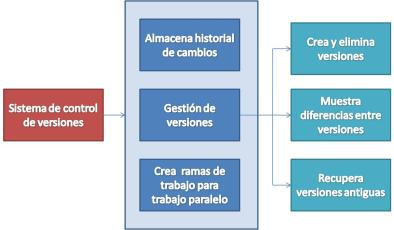
\includegraphics[width=5.5cm]{grafico1.png}	 %importamos una imagen
		\caption{ Funcionamiento de un sistema de control de	versiones}		
	\end{minipage}
	
\end{figure}

\subsection{CLASIFICACION DE LOS SISTEMAS DE CONTROL DE VERSIONES (SCV)}
Por la forma en que la información contenida en los proyectos es compartida y manipulada, los SCV se clasifican en locales, centralizados y distribuidos.Los sistemas locales se caracterizan por almacenar alguna versión del proyecto en una base de datos en el computador del desarrollador.Los sistemas centralizados se caracterizan por contar con un servidor central de donde los desarrolladores toman información de alguna versión del proyecto, la manipulan y al finalizar el proceso de desarrollo, la actualizan en el servidor central. Los sistemas distribuidos no necesitan un servidor central para almacenar la información, sino que pueden disponer de alguna versión y trabajar localmente con la
información, generando nuevas versiones, sin necesidad de almacenar la versión resultante en un
servidor central. A continuación se analizan cada una de esas clasificaciones.

\subsubsection{SCV Locales}
Los sistemas de control de versiones locales en vez de mantener las versiones como archivos independientes, los almacenaban en una base de datos. Cuando era necesario revisar una versión anterior del proyecto se usaba el sistema de control de versiones en vez de acceder directamente al archivo, de esta manera en cualquier momento solo se tenia una copia del proyecto, eliminando la posibilidad de confundir o eliminar versiones. (Medium)

\begin{figure}[h]
	\centering
	\begin{minipage}[t]{5.5cm}
		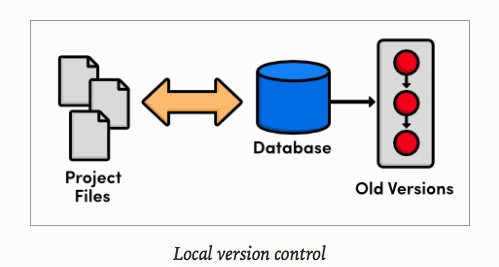
\includegraphics[width=7.5cm]{grafico5.png}	 %importamos una imagen
		\caption{ Funcionamiento de un SCV local}
	\end{minipage}
\end{figure}
%\vspace{1cm}
En este punto el control de versiones se llevaba a cabo en el computador de cada uno de los desarrolladores y no existía una manera eficiente de compartir el código entre ellos.

Una de las herramientas de control de versiones más popular fue un sistema llamado rcs, que todavía podemos encontrar en muchos de los ordenadores actuales. Hasta el famoso sistema operativo Mac OS X incluye el comando rcs cuando instalas las herramientas de desarrollo. Esta herramienta funciona básicamente guardando conjuntos de parches (es decir, las diferencias entre archivos) de una versión a otra en un formato especial en disco; puede entonces recrear cómo era un archivo en cualquier momento sumando los distintos parches.

\begin{itemize}
	\item \textbf{Revision Control System o RCS } es una implementación en software del control de versiones que automatiza las tareas de guardar, recuperar, registrar, identificar y mezclar versiones de archivos. RCS es útil para archivos que son modificados frecuentemente, por ejemplo programas informáticos, documentación, gráficos de procedimientos, monografías y cartas. RCS también puede ser utilizado para manejar archivos binarios, pero con eficacia y eficiencia reducidas. Las distintas versiones son archivadas mediante la ayuda de la herramienta diff. (Wikipedia,RCS)
	\begin{itemize}
		\item \textbf{Diff } es una utilidad para la comparación de archivos que genera las diferencias entre dos archivos o los cambios realizados en un archivo determinado comparándolo con una versión anterior del mismo archivo. Diff expone los cambios realizados por línea en los archivos de texto. Las implementaciones modernas también soportan archivos binarios. El resultado se conoce como diff o patch ya que el mismo puede ser aplicado con el programa Unix patch. (Wikipedia,Diff)
		
	\end{itemize}
	
\end{itemize}



%\vspace{1cm}
\subsubsection{SCV Centralizados}
En un SCV centralizado todas las diferentes versiones de un proyecto están almacenadas en un único repositorio de un servidor central. Para que los desarrolladores puedan acceder a esas versiones o códigos fuente deben solicitar al SCV una copia local, en la cual realizan todos los cambios necesarios, y al finalizar recurren nuevamente al SCV para que almacene las modificaciones realizadas como una nueva versión. Es entonces cuando esa versión generada estará a disposición de los demás desarrolladores, al igual que las versiones anteriores.



\begin{figure}[h]
	\centering
	\begin{minipage}[t]{5.5cm}
		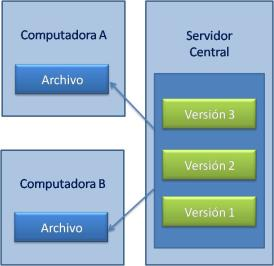
\includegraphics[width=4.5cm]{grafico2.png}	 %importamos una imagen
		\caption{ Funcionamiento de un SCV centralizado}
	\end{minipage}
	
\end{figure}
En la Figura 3 se muestra el funcionamiento de un SCV centralizado. Todos los desarrolladores trabajan sobre una rama o ramas (branches) en el mismo servidor central que aloja la última versión del proyecto. Este tipo de SCV requiere tener conexión de red para realizar las actualizaciones del servidor central (D. Otero. ,2011). Las principales aplicaciones de tipo SCV
centralizado son el CVS (CVS, 2012 ) y Subversion (Apache Subversion, 2012 ).

\begin{itemize}
	\item  \textbf{Concurrent Version System (CVS).}El CVS (CVS, 2012 ) fue por mucho tiempo la principal herramienta para el control de versiones en ambientes Open-Source. Mediante su operación en red ha soportado que múltiples desarrolladores, dispersos geográficamente, puedan compartir sus aportaciones favoreciendo el trabajo colaborativo a
	través de una arquitectura cliente-servidor. De acuerdo con Lasa (Lasa,2010) los CVS se utilizan para gestionar los cambios al código fuente del proyecto, de modo que varios desarrolladores puedan trabajar de manera coordinada sobre el mismo código fuente. Pero estos sistemas no se limitan al código fuente, también se pueden usar para todo tipo de
	documentos o archivos que estén expuestos a sufrir cambios y se requiere conservar sus diferentes versiones, o en situaciones donde varias personas trabajen en un mismo proyecto (Vesperman,2007).
	\begin{figure}[h]
		\centering
		\begin{minipage}[t]{5.5cm}
			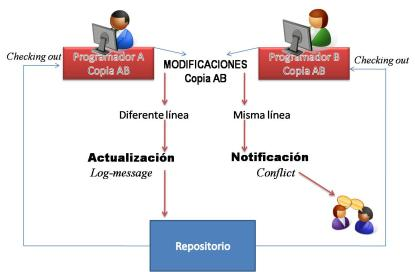
\includegraphics[width=4.5cm]{grafico4.png}	 %importamos una imagen
			\caption{ Proceso de actualización de un repositorio utilizando CVS}
		\end{minipage}
		
	\end{figure}
	
	\item \textbf{Subversion.}El sistema Subversion (Apache Subversion, 2012 ) es un SCV de código abierto (open-source), que maneja los
	cambios realizados tanto en archivos como en directorios; esto permite recuperar versiones
	anteriores de sus datos o examinar la historia de cómo cambiaron sus datos. Por otro lado, ofrece una estructura de árbol de directorios en un repositorio central; el repositorio es como un servidor de archivos excepto que recuerda todos los cambios realizados a sus archivos y directorios. Subversion permite conservar distintas versiones de
	los directorios, característica que no soporta su antecesor CVS (Lasa,2010). Además Subversion soluciona la mayoría de las deficiencias presentadas por CVS. Subversion permite al usuario obtener del repositorio una copia del proyecto, con la cual los desarrolladores trabajan en paralelo realizado sus cambios, para finalmente integrar sus copias en una versión final (F. Solsona,2007). Subversion utiliza un modelo copiar-modificar-fusionar (copy-modify-merge) como alternativa para evitar el bloqueo de archivos en el proceso de actualización. En este modelo cada usuario se conecta al repositorio del proyecto y crea una copia personal (copia espejo de los archivos y directorios contenidos en el repositorio) en la cual trabajará. Después los usuarios pueden trabajar simultáneamente modificando sus copias privadas y personales. Finalmente las copias privadas son fusionadas en una nueva versión. Subversion facilita el proceso de fusión de las diferentes copias pero el desarrollador es el responsable de que se realice correctamente esta parte del proceso (B. Collins, Fitzpatrick, C.M. Pilato,  2004 ). La forma de operar de Subversion mejora la productividad debido a que los archivos están siempre disponibles, al no bloquearlos cuando se pretendan actualizar por varios desarrolladores al mismo tiempo. La Figura 5 muestra un ejemplo del proceso de actualización en un repositorio por parte de dos desarrolladores, basado en la propuesta descrita en (B. Collins, Fitzpatrick, C.M. Pilato,  2004 ).
	
	\begin{figure}[h]
		\centering
		\begin{minipage}[t]{5.5cm}
			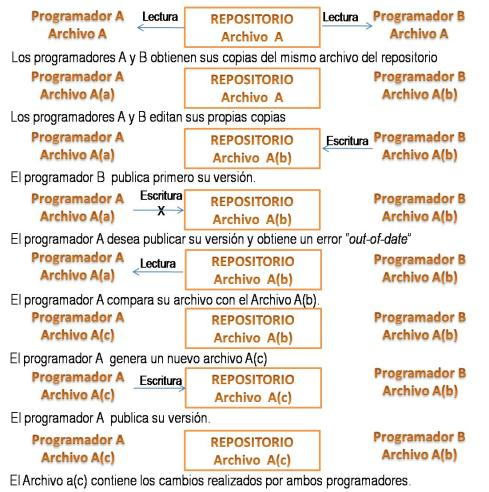
\includegraphics[width=4.5cm]{grafico6.png}	 %importamos una imagen
			\caption{ Proceso de actualización de los archivos en un repositorio utilizando Subversion}
		\end{minipage}
		
	\end{figure}
	\newpage	
	Subversion ofrece importantes ventajas con respecto a su antecesor CVS (B. Collins, Fitzpatrick, C.M. Pilato,  2004 ):	
	\begin{itemize}
		\item \textbf{Versionado de directorios.}  CVS sólo controla la
		historia de los archivos en forma individual. En
		cambio, Subversion implementa un sistema de
		archivos "virtual" de versiones que sigue los
		cambios de la estructura de directorios. Tanto a
		los directorios como a los archivos se les asigna
		una versión.
		
		
		\item \textbf{Control de historial.}  
		 Dado que CVS está limitado
		al control de versiones de archivos, no permite
		copiarlos y/o renombrarlos. Además, CVS no
		puede reemplazar un archivo versionado con otro
		que lleve el mismo nombre, sin que el nuevo
		archivo herede el historial del anterior, que tal vez
		sea completamente distinto al nuevo archivo. En
		cambio, con Subversion, se puede agregar,
		eliminar, copiar y renombrar archivos y directorios.
		Adicionalmente, cada archivo nuevo que es
		añadido inicia con un historial limpio o vacío.
		
		\item \textbf{Atomicidad.}  
		 Un conjunto de modificaciones sólo
		puede integrarse al repositorio si está totalmente
		completo. Esto permite a los programadores
		realizar cambios como unidades lógicas, lo cual
		evita los problemas que pueden ocurrir cuando
		sólo una parte de las modificaciones son enviadas
		al repositorio. El término “atómico” implica la
		indivisibilidad e irreductibilidad del proceso, ya que
		éste debe realizarse en su totalidad o de lo
		contrario no realizarse.
		
		\item \textbf{Versión en los Metadatos.} Cada directorio y
		archivo tienen un conjunto de propiedades
		asociadas, las cuales se pueden crear y
		almacenar arbitrariamente.
		
		
		\item \textbf{Conexión en diferentes capas de red.} 
		 Los
		accesos al repositorio se pueden implementar
		mediante diferentes mecanismos de red.
		Subversion puede conectarse a un servidor
		Apache usando el protocolo HTTP. Esto dota a
		Subversion de una ventaja en estabilidad e
		interoperabilidad, además de las características
		que provee el servidor Apache, tales como
		autenticación, autorización y compresión de datos.
		También una versión ligera del servidor de
		Subversion está disponible, la cual utiliza un
		protocolo propio que puede encapsularse sobre el
		protocolo SSH.
		
		\item \textbf{Manejo de datos consistente.} Subversion
		identifica las diferencias de un archivo usando un
		algoritmo de diferenciación binario, que funciona
		exactamente igual en archivos de texto (legibles) y
		archivos binarios (ilegibles por los humanos).
		Ambos tipos de archivos se almacenan
		comprimidos en el repositorio y las diferencias se
		transmiten en ambas direcciones a través de la
		red.
	\end{itemize}

	\item \textbf{Team Foundation Server.}  Microsoft Visual Studio
	Team Foundation Server  es un software
	propietario cuya plataforma de colaboración se
	encuentra en el núcleo de la solución de Visual
	Studio para la administración del ciclo de vida de
	una aplicación. Team Foundation Server (TFS)
	proporciona servicios fundamentales como control
	de versiones, seguimiento de elementos de trabajo
	y errores, automatización de la compilación y
	almacén de datos. TFS es un sistema centralizado
	que aporta una serie de herramientas que permiten
	
	colaborar y coordinar las tareas de un equipo de
	trabajo para llevar a cabo un proyecto, mejorando la
	comunicación entre los integrantes. Además,
	permite la creación de informes, implementación de
	metodologías de procesos, tendencia histórica y
	visibilidad del estado general del proyecto mediante
	un panel basado en etiquetas. Adicionalmente, se
	pueden visualizar métricas en tiempo real que
	alertan sobre potenciales problemas en etapas
	tempranas del desarrollo de software de modo que
	se puedan tomar las decisiones basadas en datos y
	aplicarse las correcciones adecuadas 
	
	TFS ofrece interfaces para facilitar la administración
	y visualización de ramas y manejo de cambios. Su
	sistema de reportes está basado en Windows
	Workflow Foundation 4.0. Otra de las características
	importantes de TSF es el almacenamiento de los
	datos del control de versiones en un servidor de
	base de datos SQL.
\end{itemize}


\subsubsection{SCV Distribuidos}
En el SCV distribuido cada desarrollador realiza una copia del repositorio de proyectos completo a su computadora, generándose un repositorio local del proyecto. Este repositorio local incluye todos los
archivos del proyecto y el historial de cambios generado en previas actualizaciones. Cuando cada
desarrollador realice modificaciones a los archivos de su repositorio local, el contenido de este repositorio se
irá distanciando de los repositorios locales de otros desarrolladores, lo que provocará que se generen
ramas de un mismo proyecto en los repositorios de cada desarrollador. De esta manera los desarrolladores pueden trabajar paralela e independientemente, guardando sus propias versiones en un repositorio local (D. Otero. ,2011). En la etapa del proceso de desarrollo del proyecto que requiera unir los repositorios locales de los desarrolladores, el SCV realizará una sincronización de copias, con lo cual se generará una nueva versión del proyecto conteniendo todos los cambios realizados por cada desarrollador. Este tipo de SCV mantiene un repositorio como referencia para realizar la sincronización de repositorios locales. En el SCV distribuido no es necesario mantener una conexión de red permanente a un servidor que contenga el repositorio de referencia, las conexiones de red por parte de los desarrolladores solo se requieren cuando se realiza el proceso de sincronización. Los principales SCV distribuidos de acuerdo a la clasificación
presentada en (B. Alwis,  J. Sillito ,2009 ) son GIT, GitHub, Mercurial, BZR, GitLab, BeetKeeper y entre otros.

\begin{figure}[h]
	\centering
	\begin{minipage}[t]{5.5cm}
		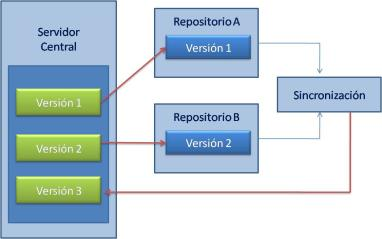
\includegraphics[width=5.5cm]{grafico3.png}	 %importamos una imagen
		\caption{ Funcionamiento de un SCV distribuido}
	\end{minipage}
	
\end{figure}
%\vspace{5cm}
En la Figura 6 se muestra brevemente el funcionamiento de un sistema de control de versiones distribuido.

\begin{itemize}
	\item \textbf{Git}. Es uno de los SCV distribuidos más populares, inicialmente desarrollado para Linux. Git permite a varios programadores trabajar paralelamente con sus propias copias de trabajo obtenidas de un repositorio, como lo efectúan todos los SCV distribuidos. Git está compuesto de una estructura de tres secciones (D. Otero. ,2011), como se describe en la Figura 7, las cuales son:
	\begin{itemize}
		\item Directorio de Git. Es donde se guardan los objetos que mantienen el historial con los cambios que se han producido en el proyecto.
		\item Directorio de trabajo. Contiene los archivos de la versión actual del proyecto sobre los que se realizan los cambios.
		\item Área de preparación o índice. Es un archivo que incluye la información de los cambios que se van a enviar en la próxima confirmación.
		\begin{figure}[h]
			\centering
			\begin{minipage}[t]{5.5cm}
				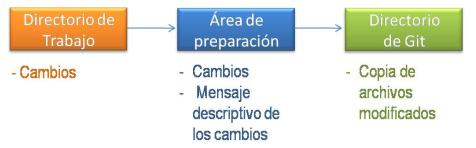
\includegraphics[width=5.5cm]{grafico7.png}	 %importamos una imagen
				\caption{Estructura de trabajo de Git}
			\end{minipage}
			
		\end{figure}
		
		
	\end{itemize}
	\newpage
	Git utiliza ramas favoreciendo el trabajo paralelo sobre un mismo proyecto. En el momento de iniciar un repositorio se genera una rama maestra, de donde se extienden nuevas ramas que incluirán todo el historial del proyecto. Cuando se han realizado los cambios en una rama, permite que ésta se combine con otras ramas, uniéndose a la rama maestra
	(merge), integrando historiales y archivos de las ramas participantes; es entonces cuando se genera una nueva versión (D. Otero. ,2011). El trabajo en ramas de Git se ilustra en la Figura 8.
	\begin{figure}[h]
		\centering
		\begin{minipage}[t]{5.5cm}
			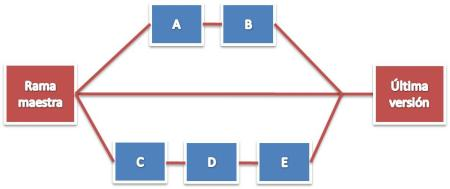
\includegraphics[width=5.5cm]{grafico8.png}	 %importamos una imagen
			\caption{Funcionamiento del trabajo en ramas de Git}
		\end{minipage}
		
	\end{figure}
	
	El proceso de actualización de los archivos contenidos en un repositorio y la posterior generación de una nueva versión utilizando Git es el siguiente: cada desarrollador debe generar una copia del repositorio original en su computadora, creando un repositorio local. Este repositorio local contiene toda la información del historial de cambios y los archivos del directorio de trabajo. En esta etapa el desarrollador puede empezar a trabajar en el repositorio Git local, creando y modificando los archivos de acuerdo a sus requerimientos.
	
	Para crear y almacenar una nueva versión el procedimiento es el siguiente: primeramente se debe consultar el estado del repositorio, con lo cual se obtiene un listado de los archivos que han sido modificados. Enseguida, se seleccionan los que se almacenarán en la nueva versión, esto es, los archivos que contienen cambios y se quieren incluir en la nueva versión. Posteriormente, se detallan los cambios que se han realizado en los archivos, esto servirá a los desarrolladores para identificar las versiones. Al finalizar estos pasos, Git almacenará en la sección "área de preparación" una nueva copia en el historial del proyecto con todos los cambios
	incluidos. Posteriormente, el desarrollador debe confirmar los cambios, con lo cual Git almacenará
	una nueva versión del proyecto en la sección ``directorio de git\''' conteniendo los archivos que sufrieron cambios y, de los archivos que no fueron modificados solo guarda el enlace al archivo anterior, que ya se encontraba en el repositorio del proyecto.
	
	En esta parte del proceso del funcionamiento de Git, los cambios y actualización de versión solo se han realizado en el repositorio local del desarrollador. Enseguida se debe realizar un proceso de fusión (merge), el cual consiste en combinar una o varias ramas de un proyecto en un repositorio local al repositorio origen o al repositorio de otros desarrolladores. La acción de merge realiza una combinación de los historiales y archivos de las dos ramas implicadas. Git detecta los cambios que existen en las dos ramas, combinándolas y generando una única versión con los cambios realizados en ambas ramas. Al efectuar el merge se cambian todos los archivos en la rama del proyecto destino, generándose una nueva versión.
	\item \textbf{GitHub } es una forja (plataforma de desarrollo colaborativo) para alojar proyectos utilizando el sistema de control de versiones Git. Utiliza el framework Ruby on Rails por GitHub, Inc. (anteriormente conocida como Logical Awesome). Desde enero de 2010, GitHub opera bajo el nombre de GitHub, Inc. El código de los proyectos alojados en GitHub se almacena típicamente de forma pública, aunque utilizando una cuenta de pago, también permite hospedar repositorios privados.
	
	\begin{itemize}
		\item Wiki para cada proyecto
		\item Página web para cada proyecto
		\item Gráfico para ver cómo los desarrolladores trabajan en sus repositorios y bifurcaciones del proyecto
		\item Funcionalidades como si se tratase de una red social, por ejemplo: seguidores;
		\item Herramienta para trabajo colaborativo entre programadores.
		\item Gestor de proyectos de estilo Kanban
	\end{itemize}
	Github hace el trabajo en equipo más ágil y sencillo, ayuda a la detección de fallos, a disminuir errores humanos, al seguimiento por etapas del proyecto, al mantenimiento de diferentes entornos, etc. (Freelancer)
	
	
	
	
	
	
	
	
	\item \textbf{Mercurial. }El SCV distribuido Mercurial  permite copiar un repositorio, conteniendo toda la historia del desarrollo del proyecto, esta copia del repositorio local funciona en forma independiente y
	autónoma sin requerir acceso a la red o a un servidor. La copia incluirá todos los archivos del proyecto y su historial. El repositorio local identifica la ubicación del repositorio origen, pero Mercurial no se comunicará con ese repositorio, a menos que el desarrollador lo realice. Mercurial tiene una interfaz de web de gran alcance que ofrece las siguientes funciones [6]: navegación sobre la estructura de repositorios, visualización del historial de cambios, despliegue del contenido de directorios y archivos, utilización de Atom y RSS para estar al tanto de los
	cambios en el repositorio, soporta usuarios remotos para copiar, modificar y actualizar repositorios.
	
	El sistema Mercurial permite, mediante una extensión convert, importar proyectos de aplicaciones como Subversion, CVS, Git, Darcs, convertiendo toda la historia del proyecto en uno nuevo en el repositorio Mercurial. Adicionalmente, la extensión convert permite exportar los cambios a Subversion, posibilitando el llevar a cabo en
	paralelo el desarrollo de un proyecto.
	
	Una de las características principales de Mercurial es su funcionamiento en línea de comandos. El proceso básico del funcionamiento de Mercurial es el siguiente: primero se debe de crear una copia local del repositorio (hg clone); el repositorio del proyecto local contendrá todos los archivos relacionados al proyecto con su registro histórico. En esta etapa el desarrollador puede iniciar los cambios o actualizaciones en los archivos del proyecto en su repositorio local, posteriormente el desarrollador puede generar una nueva revisión (hg commit) la cual incluye los archivos que han sido modificados. Enseguida el desarrollador debe autorizar los cambios, generándose una nueva versión en su repositorio local (hg push). Para integrar la nueva versión al directorio de trabajo y que pueda ser copiada por otros desarrolladores a sus repositorios locales se debe de realizar una actualización (hg update).
	
\end{itemize}

\section{SEGUNDO CAPITULO: METODOLÓGICA Y FUENTE}



Las fuente de información que elegimos son principalmente publicas y bibliográficas, porque es donde pudimos hallar mas información referente al tema.

Tambien para poder discriminar y seleccionar la información, tomamos fuentes de información primarias como ser libros,documentos,blogs y servicios web. 

Este trabajo tiene como enfoque un de tipo investigación descriptiva ya que esta refiere o narra características y propiedades de un objeto sin emplear juicios de valor y en procura de altos niveles de objetividad.

Tambien para el presente trabajo de investigación se utilizo el formato ACM y el estilo Harvard para hacer referencias a la citas bibliográficas

%\section{HALLAZGOS} 

\ 
\section{CONCLUSIONES}

\subsection{Resultados de la investigacion}

	Los sistemas de control de versiones ofrecen un soporte muy importante en el proceso de desarrollo de software, coadyuvando en la gestión del control de versiones de los archivos de código fuente e impulsando el trabajo colaborativo al permitir que múltiples desarrolladores trabajen paralelamente en un mismo proyecto en forma autónoma e independiente.
	Adicionalmente, los sistemas de control de versiones proporcionan los mecanismos para que cualquier versión de un proyecto pueda ser recuperada para visualizarse o modificarse, desplegando las diferencias entre las versiones existentes. Por otro lado, el desarrollo distribuido es soportado a través de redes de datos con diferentes mecanismos de autentificación
	
	En el presente trabajo de investigación se presentó un análisis de los sistemas de control de versiones, tanto “open-source” como propietarios, describiendo las principales funciones que ofrecen al momento de realizar una implementación y/o aplicación en el desarrollo de software.
	
	Cabe destacar que la presente investigación servirá como base para la desmostracion de una de las herramientas mas conocidad para el control de versiones basado en servicios web que es GitHub.

%\textsl{
%\lipsum[1-3]}

\section{GLOSARIO DE TÉRMINOS}
\subsection{Diccionario}
\begin{itemize}
	\item \textbf{Repositorio.- } Sitio web donde se almacena información digital. Todos los archivos almacenados son públicos y pueden ser accedidos por cualquier usuario. El tipo de información almacenada varía según el repositorio (presentaciones, imágenes, videos, documentos, etc.). (SildeShare)
	
	\item \textbf{Version.- } El versionado de software es el proceso de asignación de un nombre, código o número único, a un software para indicar su nivel de desarrollo.(Wikipedia,Version)
	
	\item \textbf{Base de Datos.- }Es una colección de información organizada de forma que un programa de ordenador pueda seleccionar rápidamente los fragmentos de datos que necesite 
	
	\item \textbf{RCS.- } Revision Control System o RCS es una implementación en software del control de versiones que automatiza las tareas de guardar, recuperar, registrar, identificar y mezclar versiones de archivos.
	
	\item \textbf{DIFF.- }es una utilidad para la comparación de archivos que genera las diferencias entre dos archivos o los cambios realizados en un archivo de-terminado comparándolo con una versión anterior del mismo archivo. Es comúnmente encontrado en los sistemas Unix como ser GNU-LINUX y MAC
	
	\item \textbf{Servidor.- } Un servidor es una aplicación en ejecución (software) capaz de atender las peticiones de un cliente y devolverle una respuesta en concordancia. Los servidores se pueden ejecutar en cualquier tipo de computadora, incluso en computadoras dedicadas a las cuales se les conoce individualmente como servidor
	
	\item \textbf{Rama.- }Una rama es una línea de desarrollo que existe de forma independiente a otra, pero
	que comparte una historia común en algún punto temporal anterior. Se puede decir que una rama
	siempre nace como una copia de algo y a partir de ahí pasa a generar su propia historia (Rosa M, 2008 )

	\item \textbf{Merge.- }	
	Una integración o fusión une dos conjuntos de cambios sobre un fichero o un conjunto de ficheros en una revisión unificada de dicho fichero o ficheros. Puede suceder cuando(libro pdf). (Rosa M, 2008 )
	
\end{itemize}

\newpage



%\subsection{La bibliografía en página aparte}

%Por ejemplo, si quiero referirme al artículo \cite{Vesperman}, o bien al libro \cite{bacaer}, lo puedo hacer escribiendo \verb|\cite{etiqueta}|.  



%\paragraph{Enlaces en la bibliografía:} Si la referencia que ponemos en la bibliografía se puede encontrar en internet, resulta interesante poner, al final, la dirección para que pueda ser consultada. Por supuesto, los enlaces que se pongan deben dirigir a páginas que cumplan con todos los requisitos legales en cuanto al respeto a los derechos de la propiedad intelectual.



\section{BLIBLIOGRAFIA}

%\renewcommand\refname{Bibliografía}



\begin{thebibliography}{9}

%\bibitem[1]{Sommerville} I. Sommerville. “Ingeniería del Software”. Pearson
%Educación, 2005.

%\bibitem[2]{Medina} F. Medina. “Marco Metodológico para la Mejora de la Eficiencia de Uso de los Procesos de Software”. Tesis Doctoral, Universidad Carlos III de Madrid, España, 2010.



\bibitem(Vesperman,2007){Vesperman} J. Vesperman. “Essential CVS”. O’Really Media Inc,
2007.

\bibitem{Lasa} M. Lasa. "Desarrollo de aplicaciones en entornos de software libre". Tesis de Maestría, Universitat Oberta de Catalunya, España, 2010

%\bibitem[5]{Rochkind} M. J. Rochkind. "The Source Code Control System",
%IEEE Transitions on Software Engineering, Vol. Se-1,
%No. 4, pp. 364-370, 1975

\bibitem[6]{Sullivan} B. O’Sullivan. “Mercurial: The Definitive Guide”. O’Really
Media Inc, 2009.

%\bibitem[7]{Koegel} M. Koegel et al. "Comparing State- and Operation- based Change Tracking on Models”. Proceedings 14th IEEE International Enterprise Distributed Object Computing, EDOC2010, pp. 163-172, 2010.

\bibitem[8]{Solsona} F. Solsona  \& E. Viso. “Manual de supervivencia en Linux”. Universidad Autónoma de México, Facultad de Ciencias, 2007.

\bibitem[9]{Otero} D. Otero. "Desarrollo de una aplicación Web para control de versiones de software". Tesis Doctoral,
Universidad Carlos III de Madrid, España, 2011.

\bibitem[10]{Alwis} B. Alwis \& J. Sillito. "Why are Software Projects Moving from Centralized to Decentralized Version Control Systems?" ICSE2009. pp. 36-39, 2009.

%\bibitem[11]{Hinsen} K. Hinsen; K. Läufer \& G. K. Thiruvathukal. "Essential Tools: Version Control Systems". Journal of IEEE Computing in Science \& Engineering, Vol. 11, No. 6, pp. 84-91, 2009

\bibitem[12]{} Concurrent Version System. Online [Feb. 2012].

\bibitem[13]{} Apache Subversion. Online [Jan. 2012].


%\bibitem[14]{Fogel}M. Bar \& K. Fogel. “Open Source Development with CVS”. Paraglyph Press, 2003.

\bibitem[15]{Fitzpatrick} B. Collins-Sussman; B. W. Fitzpatrick \& C.M. Pilato. “Version Control with Subversion”. 
2004.

%\bibitem[16]{Edgar} Edgar Tello,Claudia M,Diego A. REVISIÓN DE LOS SISTEMAS DE CONTROL DE VERSIONES UTILIZADOS EN EL DESARROLLO DE SOFTWARE. Enero-Junio 2012

%\bibitem[17]{Diana} Diana Marcela Trujillo. Sistema de Control de Versiones para el Desarrollo de Software Seguro. Fundación Universitaria los Libertadores. Agosto 2016

\bibitem{Rosa M} Rosa M. Sistemas de Control de Versiones. UNIVERSIDAD DE CÁDIZ, 2008

\bibitem[19]{Freelancer} Freelancer. Empresa de desarrollo de software.\\ https://www.freelancer.es/community/articles/github-como-puede-ayudar

\bibitem[22]{Medium}A Medium corporation\\
https://medium.com/@jointdeveloper/sistemas-de-control-de-versiones-qu\%C3\%A9-son-y-por-qu\%C3\%A9-amarlos-24b6957e716e



\bibitem[20]{Git} Git Documentacion.\\
https://git-scm.com/book/es/v1/Empezando-Acerca-del-control-de-versiones

%\bibitem[21]{Dreaming Bytes} Dreaming Bytes. Pensamientos sobre desarrollo y tecnología\\ http://www.dreamingbytes.com/como-comparar-archivos-y-carpetas-con-el-comando-diff-de-unix-mac-linux/

\bibitem[22]{SildeShare} SildeShare  \\
https://es.slideshare.net/juliocabrejos1/repositorios-definicin-caractersticas-y-ejemplos

\bibitem[22]{wikipedia} wikipedia. Enciclopedia libre\\
\textbf{GitHub} https://es.wikipedia.org/wiki/GitHub \\
\textbf{Diff} https://es.wikipedia.org/wiki/Diff \\
\textbf{RCS} https://es.wikipedia.org/wiki/Revision\_Control\_System \\ 
\textbf{Version} https://es.wikipedia.org/wiki/Versi\%C3\%B3n\_de\_software




\end{thebibliography}


\newpage

%\section*{Agradecimientos}

%Esto es por si queremos agradecer a alguien. Aunque no vamos a hacer que aparezca en el índice. 


\end{document}


%\begin{figure}%[h]
%\begin{minipage}[c]{.45\linewidth}
%	\begin{center}
%	
\includegraphics[width=5cm]{logosanmateo.png}
%	\caption{Logo San Mateo}
%   \end{center}
%\end{minipage}
%\hfill
%\begin{minipage}[c]{.45\linewidth}
%	\begin{center}
%	
\includegraphics[width=5cm]{logosanmateo.png}
%	\caption{Logo San Mateo}
%	\end{center}
%\end{minipage}
%\end{figure}



%\begin{figure}[h]
%	\centering
%	
\includegraphics[width=6cm]{logosanmateo.png}
%	\caption{El logo centrado}
%\end{figure}



%\begin{figure}%[h]
%	\begin{minipage}[c]{.45\linewidth}
%		Podemos disponer texto junto a una figura, como en este caso.		
%		También se puede hacer que la figura aparezca a la izquierda y el texto a la derecha.
%	\end{minipage}
%	\hfill
%	\begin{minipage}[c]{.45\linewidth}
%		\begin{center}
%			
\includegraphics[width=4cm]{logosanmateo.png}
%			\caption{Logo San Mateo}
%		\end{center}
%	\end{minipage}
%\end{figure}





%\bibitem[Au]{ausubel} J. H. Ausubel y P. S. Meyer. \textsl{Carrying Capacity: A Model with
%	Logistically Varying Limits, Technological Forecasting and Social Change},
%\textbf{61}, 3, (1999), pp. 209-214. http://goo.gl/Lpc4g4

%\bibitem[Al]{alvarez} N. Álvarez-Vázquez, P.A. Pérez y J. Rodríguez-Ruiz. \textsl{Métodos y
%	modelos matemáticos de la demografía}, (trabajo), Departamento de Economía
%Aplicada Cuantitativa, UNED, Málaga, 1997. http://goo.gl/n1Z2nM

%\bibitem[B]{bacaer} N. Bacaër. \textsl{A Short History of Mathematical Population Dynamics},
%Springer-Verlag, Londres, 2011. http://goo.gl/1LhzMB

%\bibitem[Ba]{banks} R. B. Banks. \textsl{Growth and Diffusion Phenomena: Mathematical
%	Frameworks and Applications}, Springer-Verlag, Berlín, 1994.

